\subsection{DRIE Etcher \#1 (DRY-Si-1)}\label{dry_DRIE_etcher}
\WaferClean

\begin{minipage}[H]{\MachinePictureWidth}
	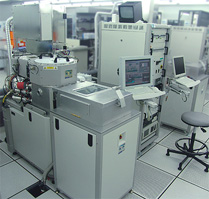
\includegraphics[width=\MachinePictureWidth]{pictures_machines/dry_DRIE.png}
\end{minipage}\begin{minipage}[H]{0.5\textwidth}
\begin{tabular}{|c|c|}
\hline
Gases available
&
C4F8, SF6, O2, N2, He \& Ar \\
\hline
RF power source
&
\makecell{1x 1000W(max) at 13.56MHz for Coil electrode,\\
1x 300W(max) at 13.56MHz for Platen electrode} \\
\hline
Electrode coolant system
&
5 to 30 \degreesC \\
\hline
High speed turbo molecular pump
&
\makecell{pumping speed of 1000 L/s at 36000 rpm \\
Fully automatic loadlock transfer system} \\
\hline
Substrate size
&
4" wafer \\
\hline
\end{tabular}

\underline{Silicon etch}

\begin{tabular}{|c|c|}
\hline
Minimum Line/Space
&
0.5 \um
\\
\hline
Low Rate Silicon Etch E/R
&
From 50nm/cycle \\
\hline
Normal Rate Silicon Etch E/R
&
Up to 2 \um/min\\
\hline
Selectivity to Photoresist
&
>50:1 \\
\hline
Selectivity to Oxide
&
>80:1 \\
\hline
Uniformity
&
7\percent \\
\hline
\end{tabular}
\end{minipage}